\documentclass[graphics]{beamer}
\usepackage{graphicx}
\usepackage{listings} % Syntax highlighing
\usepackage{fancyvrb} % Inline verbatim
\usepackage{hyperref} % Hyperlinks
\hypersetup{pdfpagemode=FullScreen}

\usepackage[normalem]{ulem}               % to striketrhourhg text
\newcommand\redout{\bgroup\markoverwith
{\textcolor{red}{\rule[0.5ex]{2pt}{0.8pt}}}\ULon}

% header in tables
\newcommand*{\thead}[1]{\multicolumn{1}{c}{\bfseries #1}}

% used for arrows from one point in the slide to another
\usepackage{tikz}
\usetikzlibrary{arrows,shapes,tikzmark}

\usetheme{Boadilla}
\title{Lecture 3: Operating Systems}
\author{UMBC CMSC 104}
\date{Th 2 Feb 2023}

\begin{document}

\begin{frame}{}
\centering
    Operating Systems
\end{frame}

\frame{\tableofcontents 
\includegraphics[scale=0.3]{L03_OperatingSystems/L3_tux.png}}

\section{What is an Operating System?}
\begin{frame}{What is an Operating System?}
    \only<1> {
        A computer program, often referred to as simply an ``OS'', which:
        \begin{itemize}
            \item Controls how the CPU, memory, and I/O devices work together to execute programs
            \item Performs many operations, such as:
            \begin{itemize}
                \item Allows you to communicate with the computer, giving it instruction via some interface.
                \item Control access (login) to the computer
                \item Keeps track of all processes currently running (and there are a lot!)
            \end{itemize}
        \end{itemize}
    }
    \only<2> {
        \begin{itemize}
            \item Provides a uniform interface for users and programs to access changing, evolving hardware (HW).
            \item Very different HW platforms can support a common OS (partially custom-written, of course). Example: regular PCs, some video game consoles, and some automotive systems run Linux.
            \item One HW platform can support multiple OSs, such as dual-booting a laptop to run Linux \textit{or} Windows.
        \end{itemize}
    }
\end{frame}

\begin{frame}{How Do I communicate with the Computer Using the OS?}
    \begin{itemize}
        \item You communicate using the particular OS' \textbf{user interface}.
        \begin{itemize}
            \item \textbf{Graphical User Interface GUI}: Point and click on Windows, Mac OS, Linux, etc.
            \item \textbf{Command Line Interface CLI}: Entering text at a prompt: Unix/Linux, Mac OS, DOS.
        \end{itemize}
        \item We will be using the Linux operating system, which is very similar to UNIX. Note that Linux has both a graphical and command-line interfaces.
    \end{itemize}
\end{frame}

\subsection{Graphical vs. Command Line Interfaces}
\begin{frame}{GUI vs. Command Line}
    \begin{itemize}
        \item We will be using the command line interface for Linux
        \item If you were to install Linux in a Virtual Machine, you could use both the GUI and CLI.
        \item All modern operating systems do allow for a mix, you can open a command line interface as a window inside a GUI.
    \end{itemize}
\end{frame}

\begin{frame}{Example of CLI}
    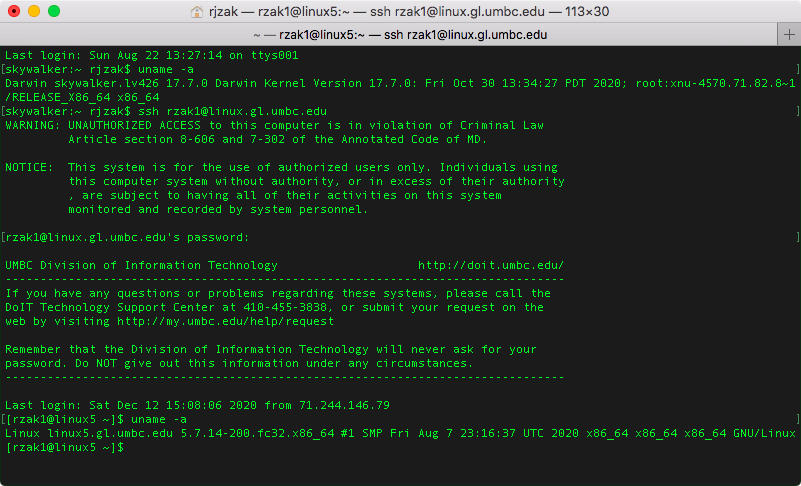
\includegraphics[scale=0.43]{L03_OperatingSystems/L3_SSH.png}
    \footnotesize{Mac OS X 10.13}
\end{frame}

\begin{frame}{Example of GUIs}
    \only<1> {
        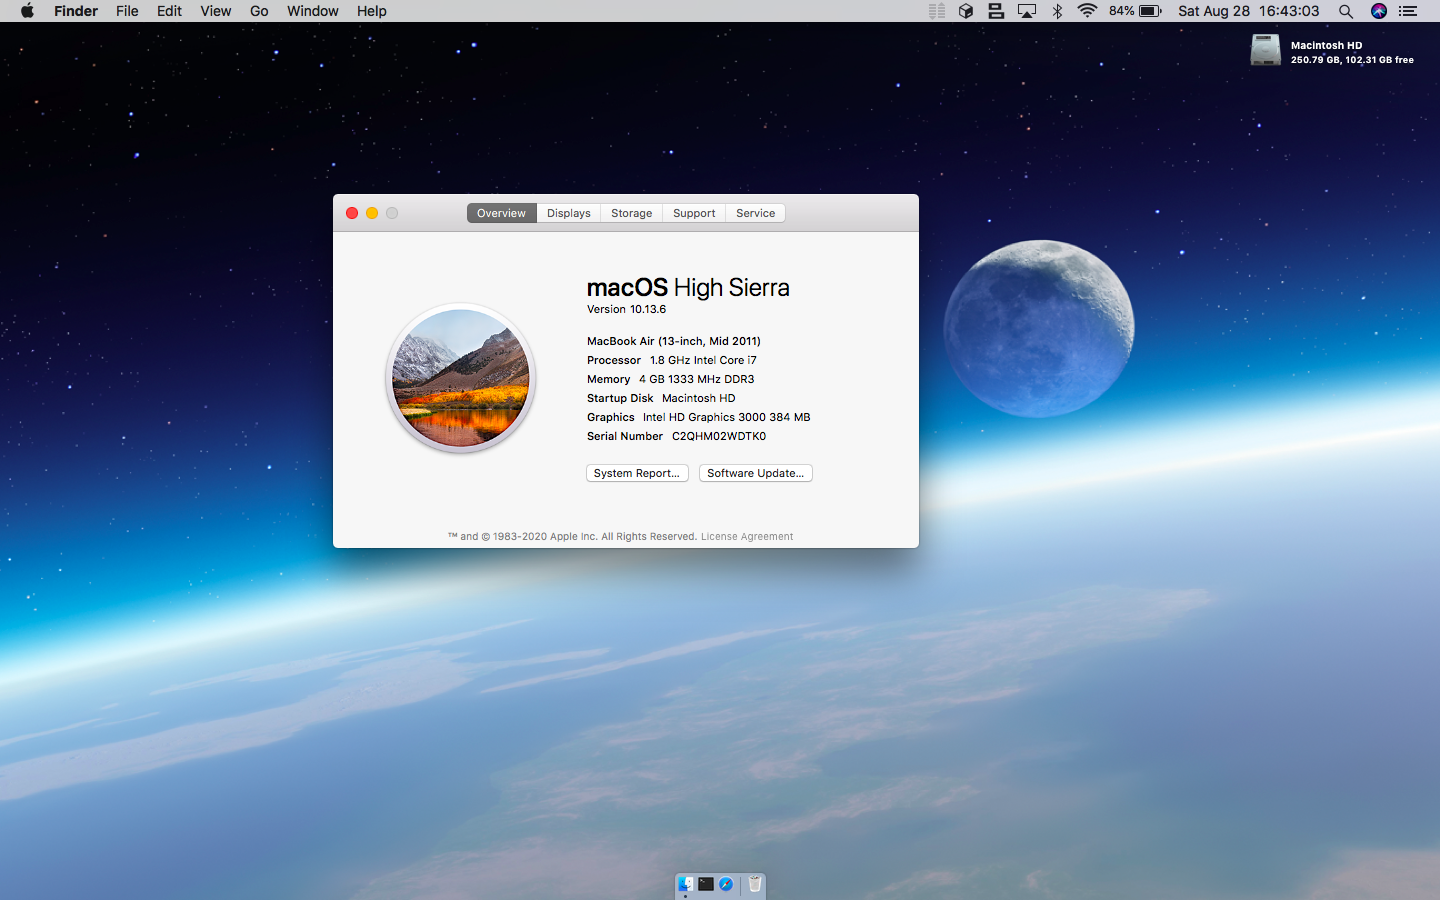
\includegraphics[scale=0.24]{L03_OperatingSystems/L3_macos.png}
        \footnotesize{Mac OS X 10.13}
    }
    \only<2> {
        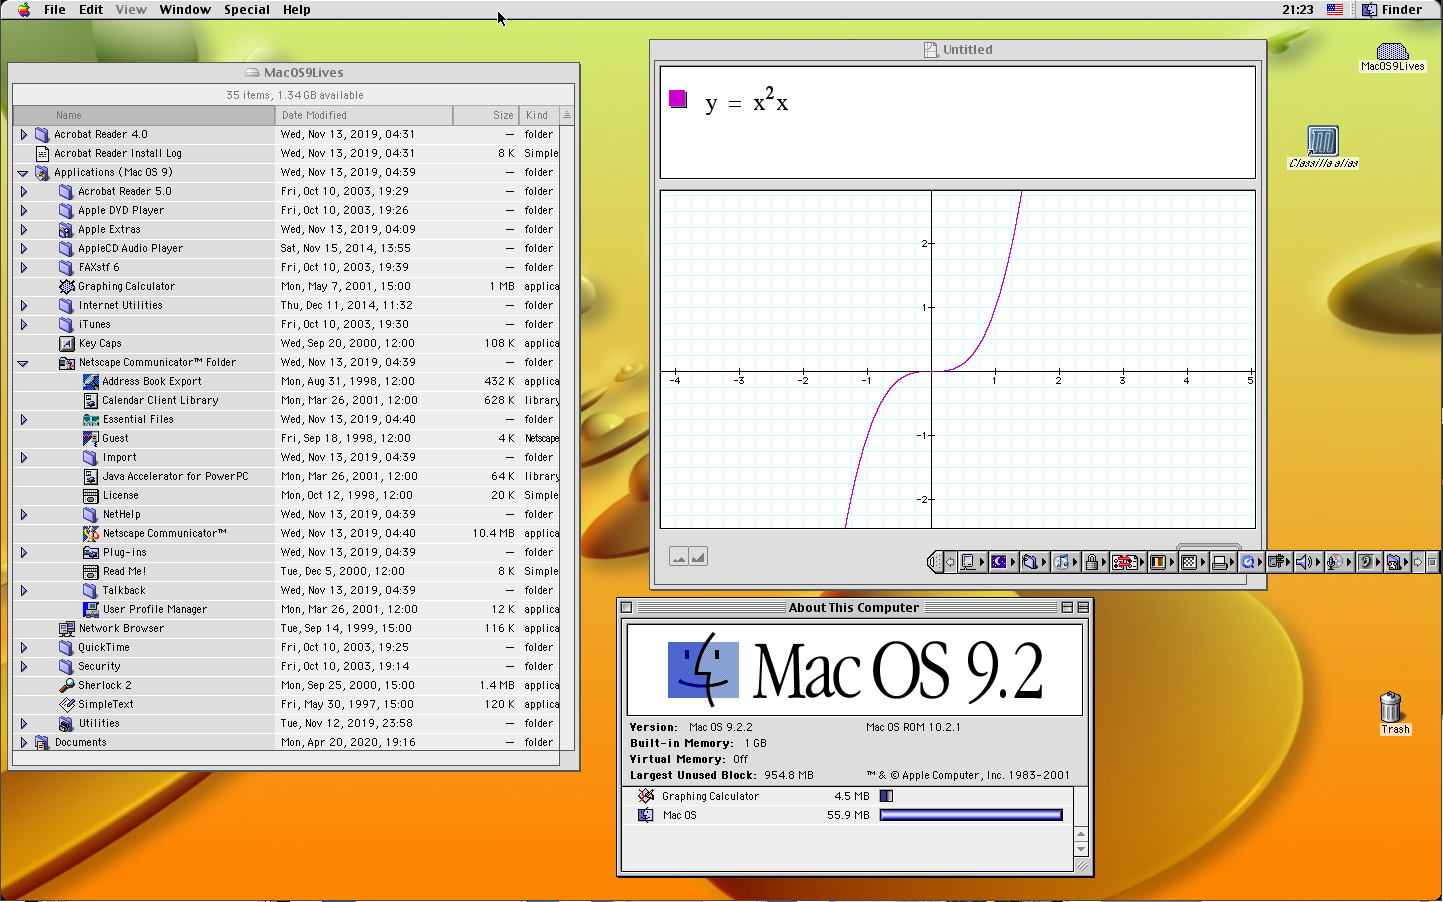
\includegraphics[scale=0.24]{L03_OperatingSystems/L03_classic_mac_os9.png}
        \footnotesize{Mac OS 9 (\href{https://en.wikipedia.org/wiki/Classic_Mac_OS}{Classic Mac OS})}
    }
    \only<3> {
        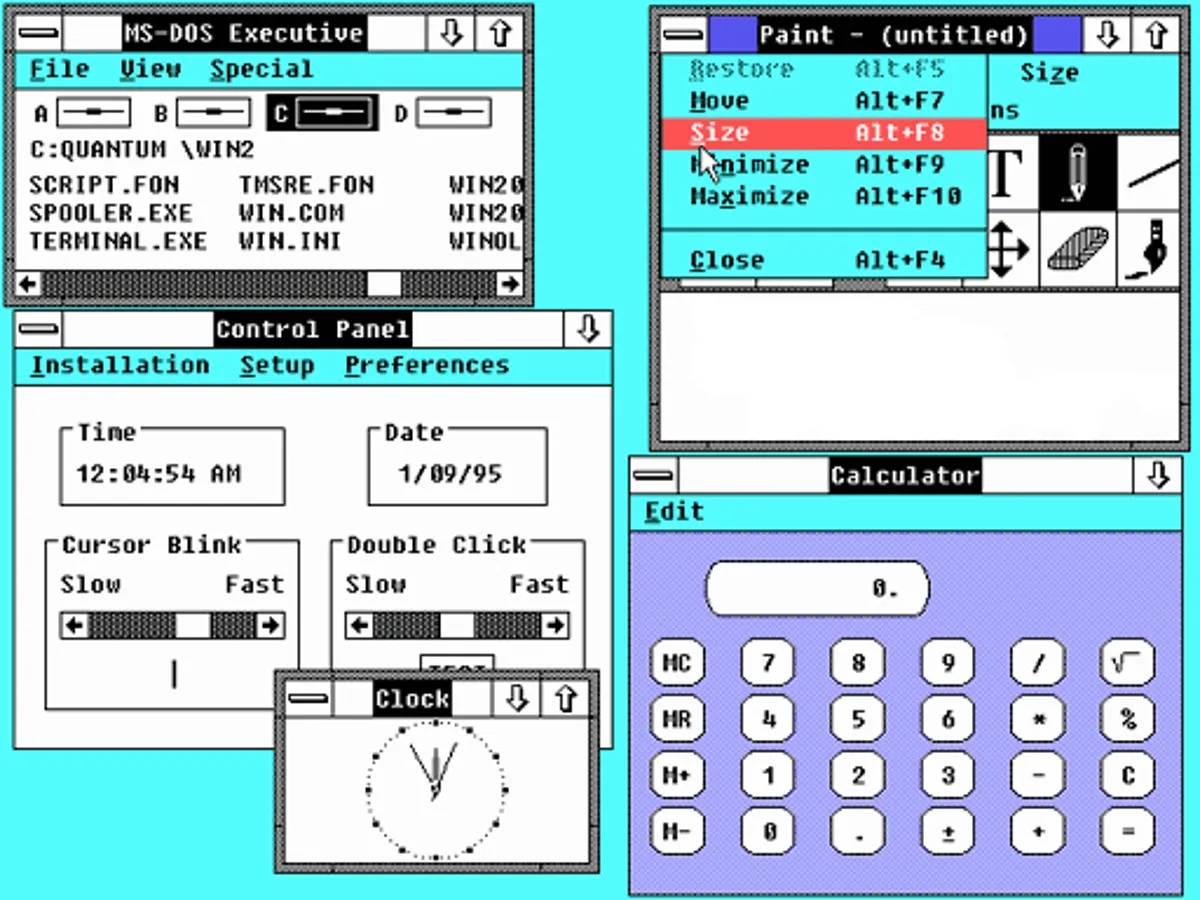
\includegraphics[scale=0.25]{L03_OperatingSystems/L03_windows2.png} \\
        \footnotesize{Windows 2.0, source \href{https://www.zdnet.com/pictures/windows-1-0-to-10-the-changing-face-of-microsofts-landmark-os/8/}{ZDnet}}
    }
    \only<4> {
        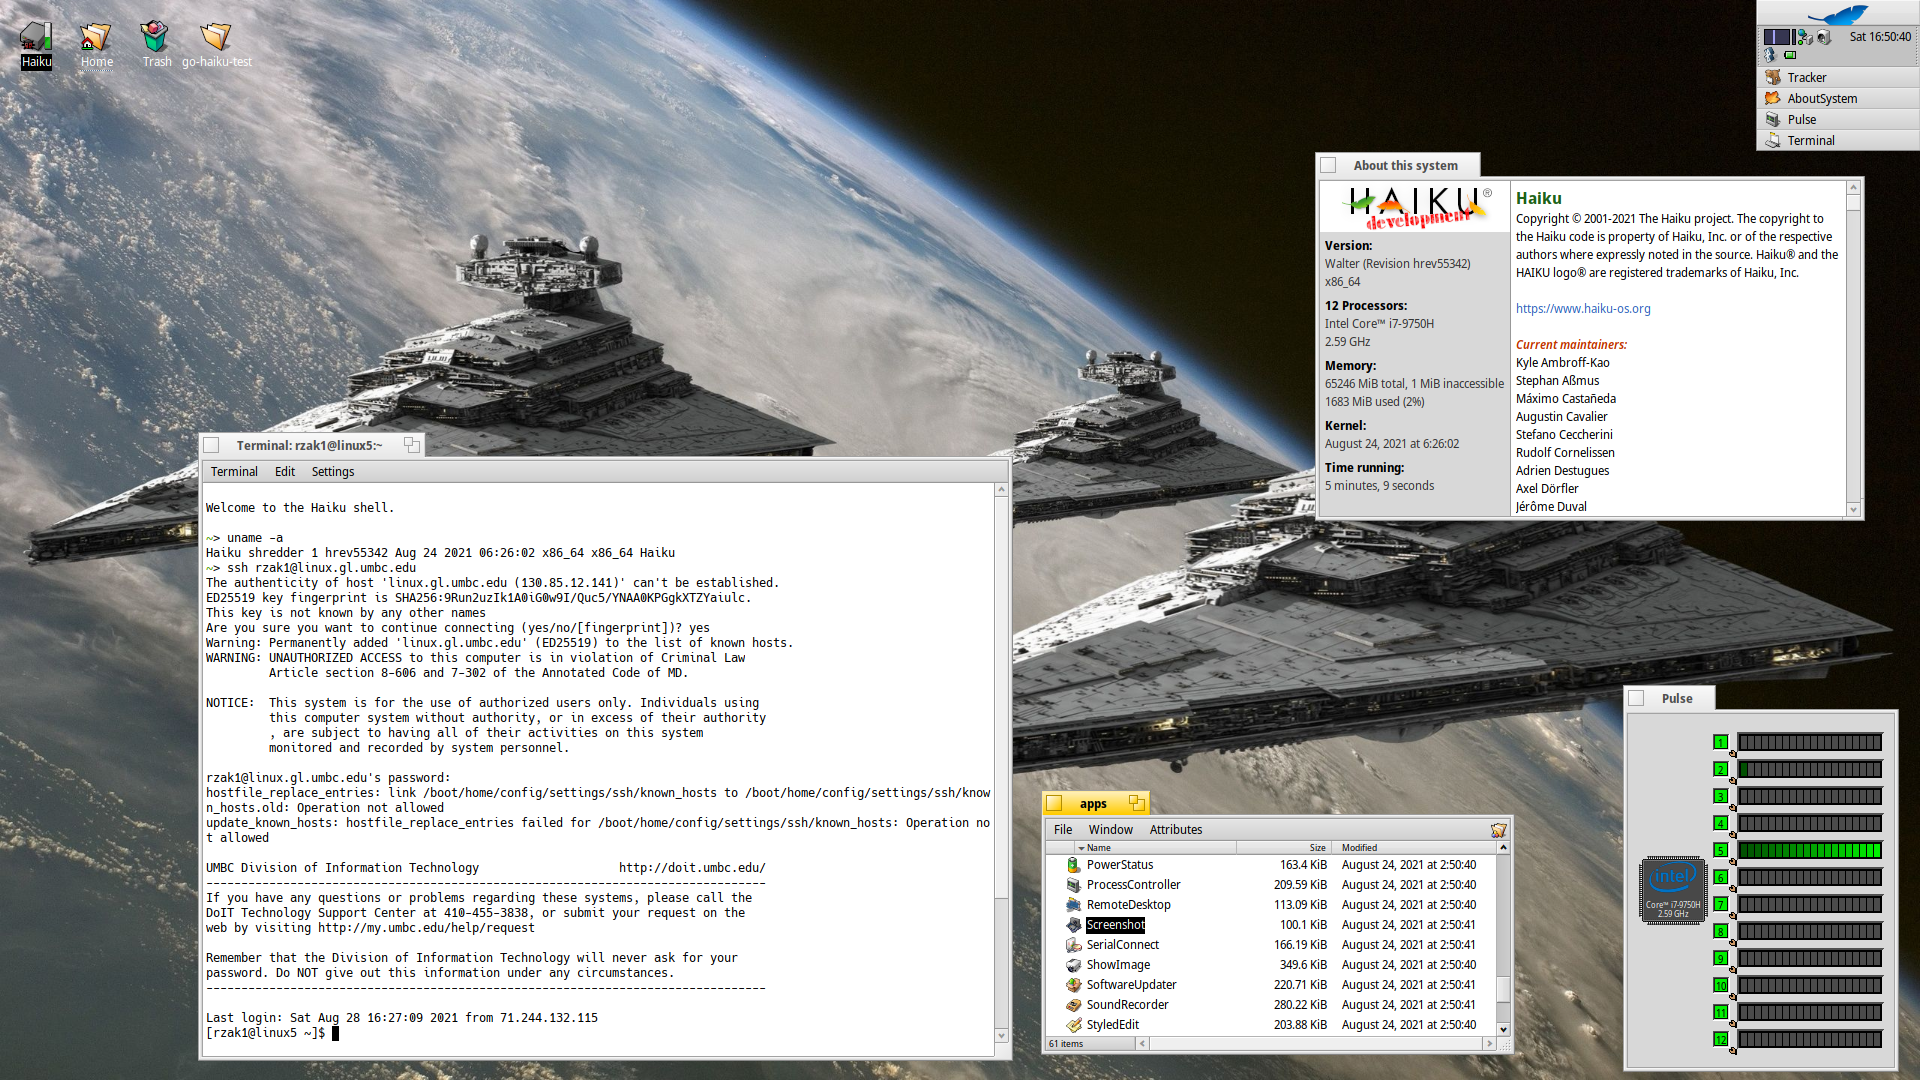
\includegraphics[scale=0.183]{L03_OperatingSystems/L3_Haiku.png}
        \footnotesize{\href{https://www.haiku-os.org/}{Haiku} R1 Beta 3}
    }
    \only<5> {
        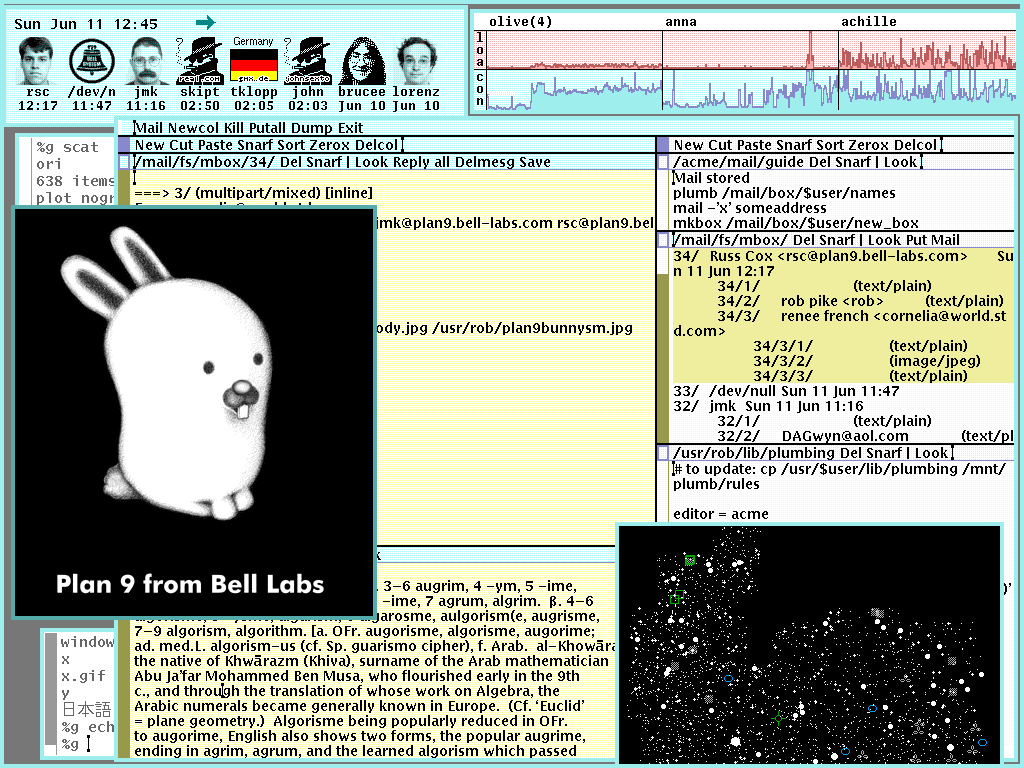
\includegraphics[scale=0.27]{L03_OperatingSystems/L03_plan9.png} \\
        \footnotesize{\href{https://en.wikipedia.org/wiki/Plan_9_from_Bell_Labs}{Plan 9}\footnote{not \href{https://en.wikipedia.org/wiki/Plan_9_from_Outer_Space}{from outer space}} from AT\&T Bell Labs}
    }
    \only<6> {
        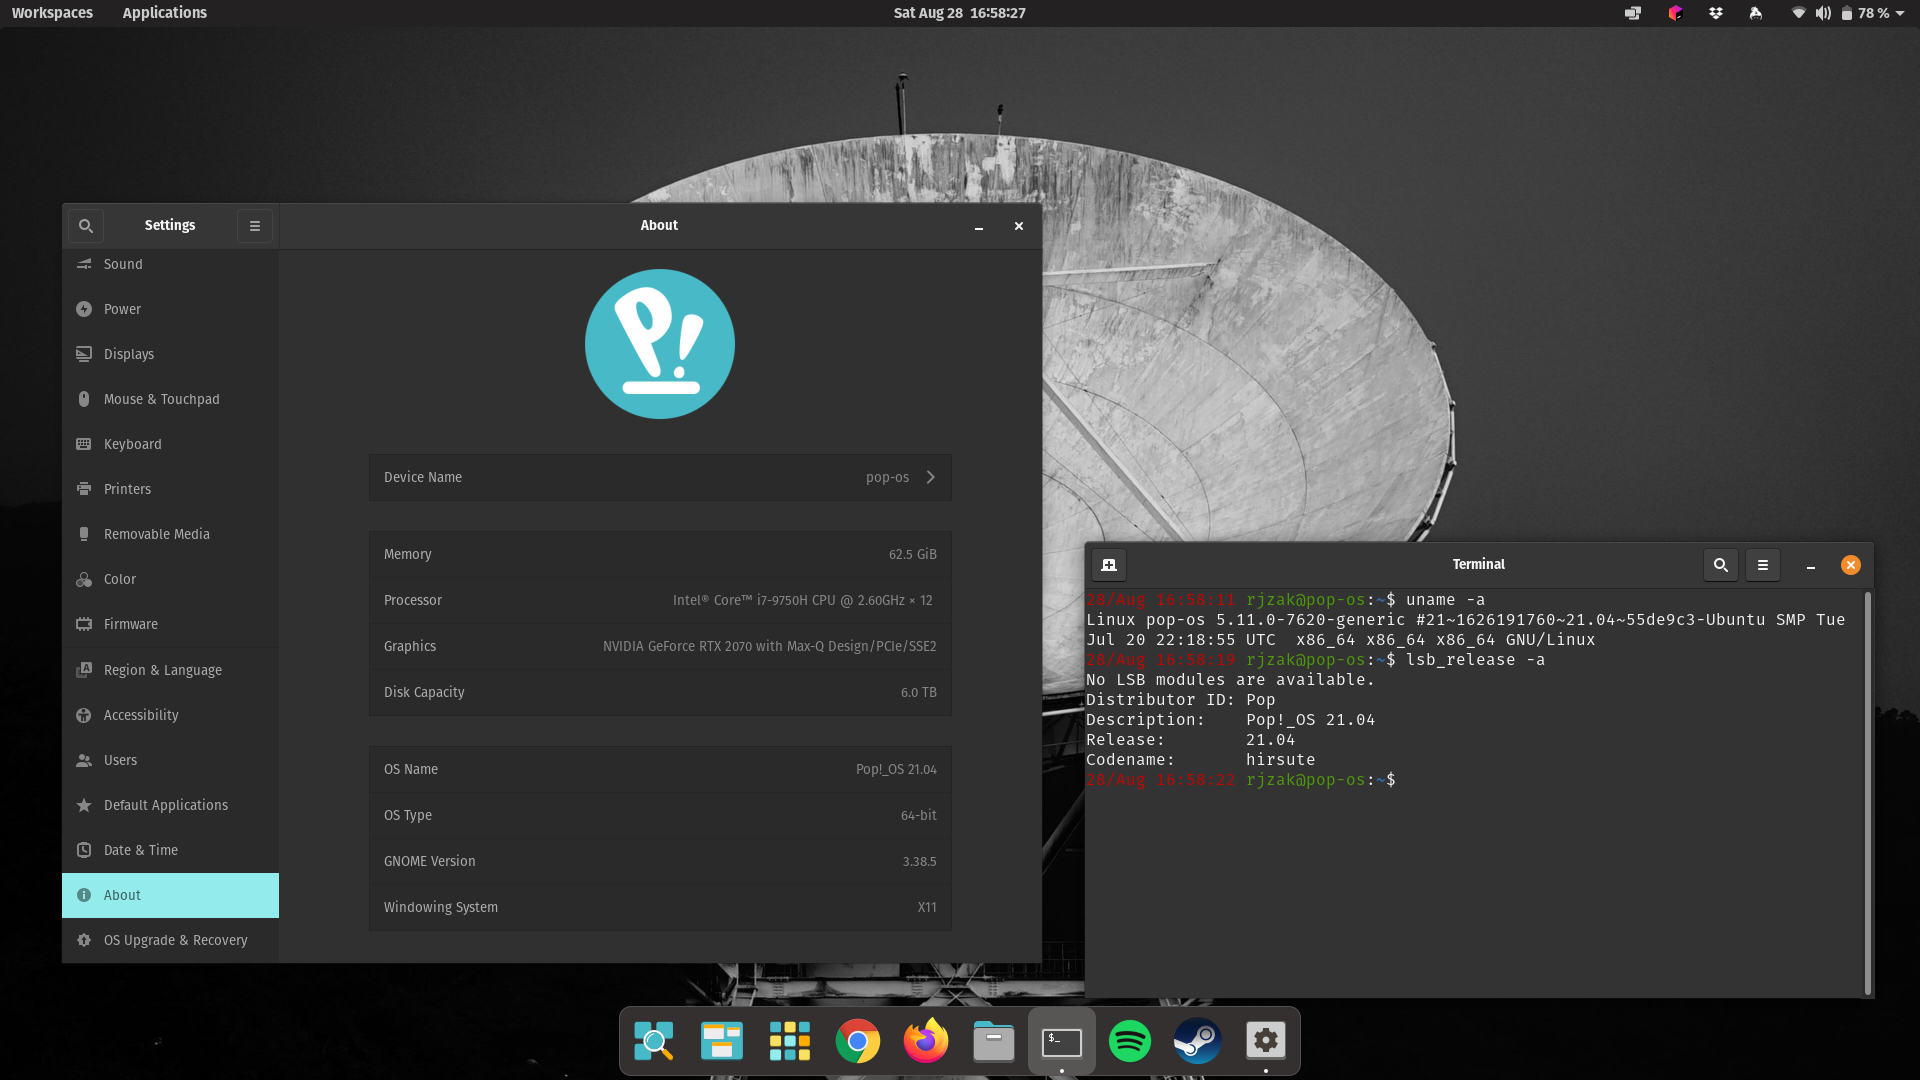
\includegraphics[scale=0.183]{L03_OperatingSystems/L03_popos.png}
        \footnotesize{\href{https://pop.system76.com/}{Pop\_OS!} 21.04 (Linux)}
    }
    \only<7> {
        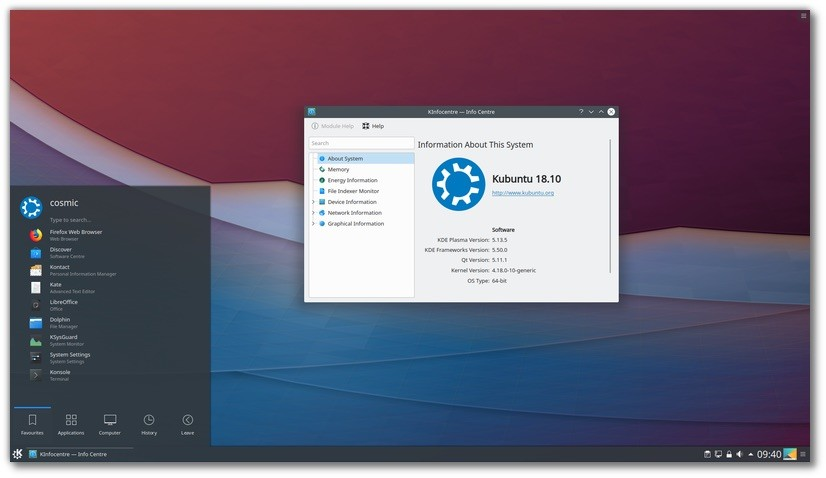
\includegraphics[scale=0.43]{L03_OperatingSystems/L3_kubuntu.jpg}
        \footnotesize{Kubuntu 18.10 (Linux)}
    }
    \only<8> {
        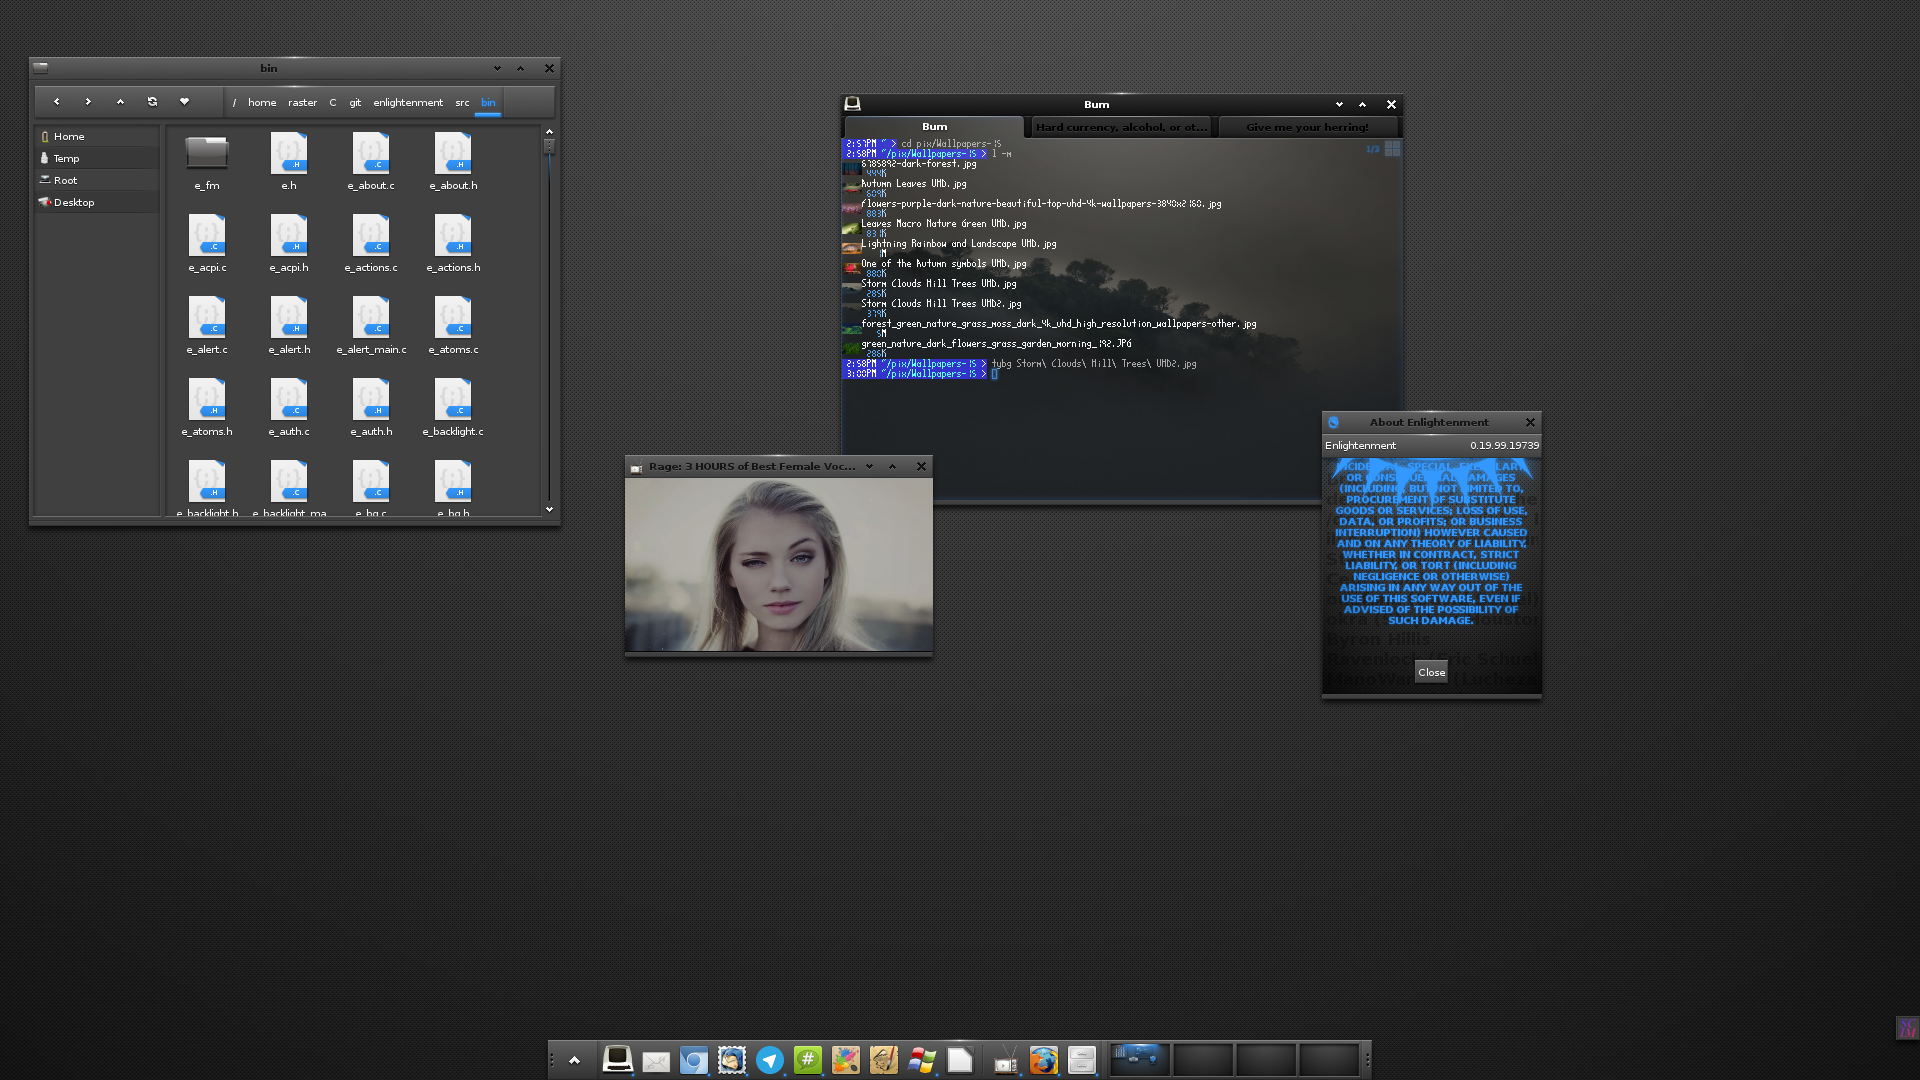
\includegraphics[scale=0.181]{L03_OperatingSystems/L3_enlightenment.png}
        \footnotesize{\href{https://www.enlightenment.org/}{Enlightenment} desktop (Linux)}
    }
\end{frame}

\begin{frame}{How Do I communicate with the Computer Using the OS? (Cont'd)}
    \begin{itemize}
        \item When you \textbf{log in} to the Linux system at UMBC, a \textbf{user prompt} is displayed: \\ \texttt{[username@linux1 \textasciitilde]\$}
        \begin{itemize}
            \item ``username'' is your UMBC username
            \item This example says ``linux1'', but could also be ``linux2'' or ``linux3''. They're all the same for our purposes. Connecting to \texttt{linux.gl.umbc.edu} randomly selects one for you.
        \end{itemize}
        \item In some cases, your prompt may look different. Ask a question if you experience any issues.
        \item The dollar sign `\$` generally means that the following text is a command on a command line interface, not that `\$` is part of the command itself.
    \end{itemize}
\end{frame}

\section{Linux Overview}
\begin{frame}{Linux Overview}
    \begin{itemize}
        \item Files and file names
        \item Directories and sub-directories
        \item Absolute and relative path names, `.' and `..'
        \item Why a command line?
        \item Frequently used commands
        \item The Shell(s)
        \item I/O Redirection
        \item Command line editing
        \item History
    \end{itemize}
\end{frame}

\begin{frame}{Files}
    \begin{itemize}
        \item A file is a sequence of bytes
        \item It can be created by any program, including the operating system
        \begin{itemize}
            \item Text or office documents
            \item Pictures and movies
            \item Programs, operating system components, drivers
        \end{itemize}
        \item A file generally contains data, like a document, or is executable code, like a program.
        \item Files are contained within directories
    \end{itemize}
\end{frame}

\begin{frame}{Linux Filenames}
    \begin{itemize}
        \item Restrictions:
        \begin{itemize}
            \item Typically do not have spaces or other reserved characters. Use '\_' instead of a space.
            \item Have a maximum length, typically 255 characters
            \item Filenames are case sensitive
        \end{itemize}
        \item For this class, use file names with letters \& numbers, and underscore '\_' or hyphen '-'. \underline{No spaces!}
        \item Some examples: firefox.exe, things2do.txt, dinner\_menu.pdf, fav\_song.mp3
        \item Not all files have an extension, so use the `file` command to see what type of file it is.
    \end{itemize}
\end{frame}

\subsection{Directories}
\begin{frame}{Directories}
    \begin{itemize}
        \item Directories contain files and other directories, called \textbf{subdirectories}. They may also be empty.
        \item Directories are organized in a hierarchical fashion.
        \item They are important in keeping files organized.
    \end{itemize}
\end{frame}

\begin{frame}{Example Directory Tree}
    % Graphic for TeX using PGF
% Title: /home/rjzak/Diagram1.dia
% Creator: Dia v0.97+git
% CreationDate: Sat Aug 28 17:58:21 2021
% For: rjzak
% \usepackage{tikz}
% The following commands are not supported in PSTricks at present
% We define them conditionally, so when they are implemented,
% this pgf file will use them.
\ifx\du\undefined
  \newlength{\du}
\fi
\setlength{\du}{15\unitlength}
\begin{tikzpicture}[even odd rule]
\pgftransformxscale{1.000000}
\pgftransformyscale{-1.000000}
\definecolor{dialinecolor}{rgb}{0.000000, 0.000000, 0.000000}
\pgfsetstrokecolor{dialinecolor}
\pgfsetstrokeopacity{1.000000}
\definecolor{diafillcolor}{rgb}{1.000000, 1.000000, 1.000000}
\pgfsetfillcolor{diafillcolor}
\pgfsetfillopacity{1.000000}
% setfont left to latex
\definecolor{dialinecolor}{rgb}{0.000000, 0.000000, 0.000000}
\pgfsetstrokecolor{dialinecolor}
\pgfsetstrokeopacity{1.000000}
\definecolor{diafillcolor}{rgb}{0.000000, 0.000000, 0.000000}
\pgfsetfillcolor{diafillcolor}
\pgfsetfillopacity{1.000000}
\node[anchor=base west,inner sep=0pt,outer sep=0pt,color=dialinecolor] at (2.400000\du,0.750000\du){/afs/umbc.edu/users/j/d/jdoe28/home/};
% setfont left to latex
\definecolor{dialinecolor}{rgb}{0.000000, 0.000000, 0.000000}
\pgfsetstrokecolor{dialinecolor}
\pgfsetstrokeopacity{1.000000}
\definecolor{diafillcolor}{rgb}{0.000000, 0.000000, 0.000000}
\pgfsetfillcolor{diafillcolor}
\pgfsetfillopacity{1.000000}
\node[anchor=base west,inner sep=0pt,outer sep=0pt,color=dialinecolor] at (1.050000\du,2.900000\du){Mail/};
% setfont left to latex
\definecolor{dialinecolor}{rgb}{0.000000, 0.000000, 0.000000}
\pgfsetstrokecolor{dialinecolor}
\pgfsetstrokeopacity{1.000000}
\definecolor{diafillcolor}{rgb}{0.000000, 0.000000, 0.000000}
\pgfsetfillcolor{diafillcolor}
\pgfsetfillopacity{1.000000}
\node[anchor=base west,inner sep=0pt,outer sep=0pt,color=dialinecolor] at (5.050000\du,2.900000\du){recipes/};
% setfont left to latex
\definecolor{dialinecolor}{rgb}{0.000000, 0.000000, 0.000000}
\pgfsetstrokecolor{dialinecolor}
\pgfsetstrokeopacity{1.000000}
\definecolor{diafillcolor}{rgb}{0.000000, 0.000000, 0.000000}
\pgfsetfillcolor{diafillcolor}
\pgfsetfillopacity{1.000000}
\node[anchor=base west,inner sep=0pt,outer sep=0pt,color=dialinecolor] at (12.200000\du,2.950000\du){courses/};
% setfont left to latex
\definecolor{dialinecolor}{rgb}{0.000000, 0.000000, 0.000000}
\pgfsetstrokecolor{dialinecolor}
\pgfsetstrokeopacity{1.000000}
\definecolor{diafillcolor}{rgb}{0.000000, 0.000000, 0.000000}
\pgfsetfillcolor{diafillcolor}
\pgfsetfillopacity{1.000000}
\node[anchor=base west,inner sep=0pt,outer sep=0pt,color=dialinecolor] at (14.300000\du,4.600000\du){CMSC104};
% setfont left to latex
\definecolor{dialinecolor}{rgb}{0.000000, 0.000000, 0.000000}
\pgfsetstrokecolor{dialinecolor}
\pgfsetstrokeopacity{1.000000}
\definecolor{diafillcolor}{rgb}{0.000000, 0.000000, 0.000000}
\pgfsetfillcolor{diafillcolor}
\pgfsetfillopacity{1.000000}
\node[anchor=base west,inner sep=0pt,outer sep=0pt,color=dialinecolor] at (4.100000\du,4.600000\du){pies/};
% setfont left to latex
\definecolor{dialinecolor}{rgb}{0.000000, 0.000000, 0.000000}
\pgfsetstrokecolor{dialinecolor}
\pgfsetstrokeopacity{1.000000}
\definecolor{diafillcolor}{rgb}{0.000000, 0.000000, 0.000000}
\pgfsetfillcolor{diafillcolor}
\pgfsetfillopacity{1.000000}
\node[anchor=base west,inner sep=0pt,outer sep=0pt,color=dialinecolor] at (7.650000\du,4.550000\du){cookies/};
% setfont left to latex
\definecolor{dialinecolor}{rgb}{0.000000, 0.000000, 0.000000}
\pgfsetstrokecolor{dialinecolor}
\pgfsetstrokeopacity{1.000000}
\definecolor{diafillcolor}{rgb}{0.000000, 0.000000, 0.000000}
\pgfsetfillcolor{diafillcolor}
\pgfsetfillopacity{1.000000}
\node[anchor=base west,inner sep=0pt,outer sep=0pt,color=dialinecolor] at (0.400000\du,6.800000\du){apple.txt};
% setfont left to latex
\definecolor{dialinecolor}{rgb}{0.000000, 0.000000, 0.000000}
\pgfsetstrokecolor{dialinecolor}
\pgfsetstrokeopacity{1.000000}
\definecolor{diafillcolor}{rgb}{0.000000, 0.000000, 0.000000}
\pgfsetfillcolor{diafillcolor}
\pgfsetfillopacity{1.000000}
\node[anchor=base west,inner sep=0pt,outer sep=0pt,color=dialinecolor] at (4.400000\du,6.700000\du){pumpkin.txt};
% setfont left to latex
\definecolor{dialinecolor}{rgb}{0.000000, 0.000000, 0.000000}
\pgfsetstrokecolor{dialinecolor}
\pgfsetstrokeopacity{1.000000}
\definecolor{diafillcolor}{rgb}{0.000000, 0.000000, 0.000000}
\pgfsetfillcolor{diafillcolor}
\pgfsetfillopacity{1.000000}
\node[anchor=base west,inner sep=0pt,outer sep=0pt,color=dialinecolor] at (11.000000\du,6.750000\du){choc\_chip.txt};
\pgfsetlinewidth{0.100000\du}
\pgfsetdash{}{0pt}
\pgfsetbuttcap
{
\definecolor{diafillcolor}{rgb}{0.000000, 0.000000, 0.000000}
\pgfsetfillcolor{diafillcolor}
\pgfsetfillopacity{1.000000}
% was here!!!
\pgfsetarrowsend{stealth}
\definecolor{dialinecolor}{rgb}{0.000000, 0.000000, 0.000000}
\pgfsetstrokecolor{dialinecolor}
\pgfsetstrokeopacity{1.000000}
\draw (7.900000\du,0.900000\du)--(2.800000\du,2.450000\du);
}
\pgfsetlinewidth{0.100000\du}
\pgfsetdash{}{0pt}
\pgfsetbuttcap
{
\definecolor{diafillcolor}{rgb}{0.000000, 0.000000, 0.000000}
\pgfsetfillcolor{diafillcolor}
\pgfsetfillopacity{1.000000}
% was here!!!
\pgfsetarrowsend{stealth}
\definecolor{dialinecolor}{rgb}{0.000000, 0.000000, 0.000000}
\pgfsetstrokecolor{dialinecolor}
\pgfsetstrokeopacity{1.000000}
\draw (8.150000\du,0.750000\du)--(7.550000\du,2.300000\du);
}
\pgfsetlinewidth{0.100000\du}
\pgfsetdash{}{0pt}
\pgfsetbuttcap
{
\definecolor{diafillcolor}{rgb}{0.000000, 0.000000, 0.000000}
\pgfsetfillcolor{diafillcolor}
\pgfsetfillopacity{1.000000}
% was here!!!
\pgfsetarrowsend{stealth}
\definecolor{dialinecolor}{rgb}{0.000000, 0.000000, 0.000000}
\pgfsetstrokecolor{dialinecolor}
\pgfsetstrokeopacity{1.000000}
\draw (8.100000\du,0.800000\du)--(12.450000\du,2.450000\du);
}
\pgfsetlinewidth{0.100000\du}
\pgfsetdash{}{0pt}
\pgfsetbuttcap
{
\definecolor{diafillcolor}{rgb}{0.000000, 0.000000, 0.000000}
\pgfsetfillcolor{diafillcolor}
\pgfsetfillopacity{1.000000}
% was here!!!
\pgfsetarrowsend{stealth}
\definecolor{dialinecolor}{rgb}{0.000000, 0.000000, 0.000000}
\pgfsetstrokecolor{dialinecolor}
\pgfsetstrokeopacity{1.000000}
\draw (6.300000\du,2.950000\du)--(5.500000\du,3.900000\du);
}
\pgfsetlinewidth{0.100000\du}
\pgfsetdash{}{0pt}
\pgfsetbuttcap
{
\definecolor{diafillcolor}{rgb}{0.000000, 0.000000, 0.000000}
\pgfsetfillcolor{diafillcolor}
\pgfsetfillopacity{1.000000}
% was here!!!
\pgfsetarrowsend{stealth}
\definecolor{dialinecolor}{rgb}{0.000000, 0.000000, 0.000000}
\pgfsetstrokecolor{dialinecolor}
\pgfsetstrokeopacity{1.000000}
\draw (6.400000\du,3.000000\du)--(8.050000\du,4.150000\du);
}
\pgfsetlinewidth{0.100000\du}
\pgfsetdash{}{0pt}
\pgfsetbuttcap
{
\definecolor{diafillcolor}{rgb}{0.000000, 0.000000, 0.000000}
\pgfsetfillcolor{diafillcolor}
\pgfsetfillopacity{1.000000}
% was here!!!
\pgfsetarrowsend{stealth}
\definecolor{dialinecolor}{rgb}{0.000000, 0.000000, 0.000000}
\pgfsetstrokecolor{dialinecolor}
\pgfsetstrokeopacity{1.000000}
\draw (13.600000\du,3.150000\du)--(14.850000\du,4.000000\du);
}
\pgfsetlinewidth{0.100000\du}
\pgfsetdash{}{0pt}
\pgfsetbuttcap
{
\definecolor{diafillcolor}{rgb}{0.000000, 0.000000, 0.000000}
\pgfsetfillcolor{diafillcolor}
\pgfsetfillopacity{1.000000}
% was here!!!
\pgfsetarrowsend{stealth}
\definecolor{dialinecolor}{rgb}{0.000000, 0.000000, 0.000000}
\pgfsetstrokecolor{dialinecolor}
\pgfsetstrokeopacity{1.000000}
\draw (4.700000\du,4.650000\du)--(6.500000\du,6.150000\du);
}
\pgfsetlinewidth{0.100000\du}
\pgfsetdash{}{0pt}
\pgfsetbuttcap
{
\definecolor{diafillcolor}{rgb}{0.000000, 0.000000, 0.000000}
\pgfsetfillcolor{diafillcolor}
\pgfsetfillopacity{1.000000}
% was here!!!
\pgfsetarrowsend{stealth}
\definecolor{dialinecolor}{rgb}{0.000000, 0.000000, 0.000000}
\pgfsetstrokecolor{dialinecolor}
\pgfsetstrokeopacity{1.000000}
\draw (4.650000\du,4.700000\du)--(2.800000\du,6.050000\du);
}
\pgfsetlinewidth{0.100000\du}
\pgfsetdash{}{0pt}
\pgfsetbuttcap
{
\definecolor{diafillcolor}{rgb}{0.000000, 0.000000, 0.000000}
\pgfsetfillcolor{diafillcolor}
\pgfsetfillopacity{1.000000}
% was here!!!
\pgfsetarrowsend{stealth}
\definecolor{dialinecolor}{rgb}{0.000000, 0.000000, 0.000000}
\pgfsetstrokecolor{dialinecolor}
\pgfsetstrokeopacity{1.000000}
\draw (9.900000\du,4.700000\du)--(12.350000\du,6.250000\du);
}
\end{tikzpicture}

\end{frame}

\begin{frame}{More Directories}
    \begin{itemize}
        \item Your \textbf{home directory} is where you are located when you log in, eg: /afs/umbc.edu/home/u/s/username/home/. This is where you can save files, it's your space.
        \item The \textbf{current directory} is where you are located at any time while you are using the system. Sometimes it shows in your \textbf{command} or \textbf{user prompt}, and you can easily figure it out by running \texttt{pwd}.
        \item The \textbf{/} (pronounced ``slash'') is the root directory in Linux, analogous to \texttt{C:\textbackslash} in Windows.
        \item File in the same directory must have unique names.
        \item \textbf{Paths} allow us to have the same name to different files located in different directories.
        \item Each running program has a current directory (just like a user), and all file names are implicitly assumed to be in that directory, unless they have a slash.
    \end{itemize}
\end{frame}

\begin{frame}{Absolute Path}
    \begin{itemize}
        \item The \textbf{absolute path} is the path which contains the direct directory \& all subdirectories needed to reach the file.
        \item It points to the same file regardless of the current working directory.
        \item Example: \texttt{/afs/umbc.edu/j/d/jdoe28/home/recipes/pies/pumpkin.txt}
    \end{itemize}
\end{frame}

\begin{frame}{Relative Path}
    \begin{itemize}
        \item The relative path is a partial path to a file in relation to the current working directory.
        \item If inside the home directory for \texttt{jdoe28}, the relative path for the same file would be: \texttt{recipes/pies/apple.txt}
    \end{itemize}
\end{frame}

\begin{frame}{Subdirectories}
    \begin{itemize}
        \item Are used for organizing your files.
        \item Example:
        \begin{itemize}
            \item Make a subdirectory for CMSC104
            \item Make subdirectories for each assignment
        \end{itemize}
    \end{itemize}
    \centering
    % Graphic for TeX using PGF
% Title: /home/rjzak/Diagram1.dia
% Creator: Dia v0.97+git
% CreationDate: Sat Aug 28 18:22:01 2021
% For: rjzak
% \usepackage{tikz}
% The following commands are not supported in PSTricks at present
% We define them conditionally, so when they are implemented,
% this pgf file will use them.
\ifx\du\undefined
  \newlength{\du}
\fi
\setlength{\du}{15\unitlength}
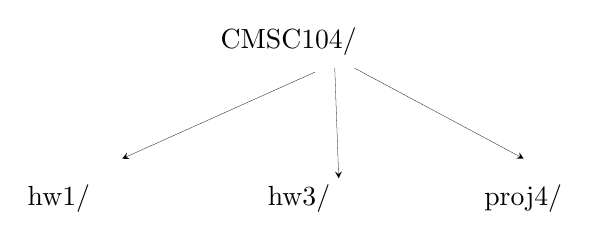
\begin{tikzpicture}[even odd rule]
\pgftransformxscale{1.000000}
\pgftransformyscale{-1.000000}
\definecolor{dialinecolor}{rgb}{0.000000, 0.000000, 0.000000}
\pgfsetstrokecolor{dialinecolor}
\pgfsetstrokeopacity{1.000000}
\definecolor{diafillcolor}{rgb}{1.000000, 1.000000, 1.000000}
\pgfsetfillcolor{diafillcolor}
\pgfsetfillopacity{1.000000}
% setfont left to latex
\definecolor{dialinecolor}{rgb}{0.000000, 0.000000, 0.000000}
\pgfsetstrokecolor{dialinecolor}
\pgfsetstrokeopacity{1.000000}
\definecolor{diafillcolor}{rgb}{0.000000, 0.000000, 0.000000}
\pgfsetfillcolor{diafillcolor}
\pgfsetfillopacity{1.000000}
\node[anchor=base west,inner sep=0pt,outer sep=0pt,color=dialinecolor] at (5.450000\du,0.950000\du){CMSC104/};
% setfont left to latex
\definecolor{dialinecolor}{rgb}{0.000000, 0.000000, 0.000000}
\pgfsetstrokecolor{dialinecolor}
\pgfsetstrokeopacity{1.000000}
\definecolor{diafillcolor}{rgb}{0.000000, 0.000000, 0.000000}
\pgfsetfillcolor{diafillcolor}
\pgfsetfillopacity{1.000000}
\node[anchor=base west,inner sep=0pt,outer sep=0pt,color=dialinecolor] at (3.000000\du,2.950000\du){hw1/};
% setfont left to latex
\definecolor{dialinecolor}{rgb}{0.000000, 0.000000, 0.000000}
\pgfsetstrokecolor{dialinecolor}
\pgfsetstrokeopacity{1.000000}
\definecolor{diafillcolor}{rgb}{0.000000, 0.000000, 0.000000}
\pgfsetfillcolor{diafillcolor}
\pgfsetfillopacity{1.000000}
\node[anchor=base west,inner sep=0pt,outer sep=0pt,color=dialinecolor] at (6.050000\du,2.950000\du){hw3/};
% setfont left to latex
\definecolor{dialinecolor}{rgb}{0.000000, 0.000000, 0.000000}
\pgfsetstrokecolor{dialinecolor}
\pgfsetstrokeopacity{1.000000}
\definecolor{diafillcolor}{rgb}{0.000000, 0.000000, 0.000000}
\pgfsetfillcolor{diafillcolor}
\pgfsetfillopacity{1.000000}
\node[anchor=base west,inner sep=0pt,outer sep=0pt,color=dialinecolor] at (8.800000\du,2.950000\du){proj4/};
\pgfsetlinewidth{0.100000\du}
\pgfsetdash{}{0pt}
\pgfsetbuttcap
{
\definecolor{diafillcolor}{rgb}{0.000000, 0.000000, 0.000000}
\pgfsetfillcolor{diafillcolor}
\pgfsetfillopacity{1.000000}
% was here!!!
\pgfsetarrowsend{stealth}
\definecolor{dialinecolor}{rgb}{0.000000, 0.000000, 0.000000}
\pgfsetstrokecolor{dialinecolor}
\pgfsetstrokeopacity{1.000000}
\draw (6.650000\du,1.250000\du)--(4.200000\du,2.350000\du);
}
\pgfsetlinewidth{0.100000\du}
\pgfsetdash{}{0pt}
\pgfsetbuttcap
{
\definecolor{diafillcolor}{rgb}{0.000000, 0.000000, 0.000000}
\pgfsetfillcolor{diafillcolor}
\pgfsetfillopacity{1.000000}
% was here!!!
\pgfsetarrowsend{stealth}
\definecolor{dialinecolor}{rgb}{0.000000, 0.000000, 0.000000}
\pgfsetstrokecolor{dialinecolor}
\pgfsetstrokeopacity{1.000000}
\draw (6.900000\du,1.200000\du)--(6.950000\du,2.600000\du);
}
\pgfsetlinewidth{0.100000\du}
\pgfsetdash{}{0pt}
\pgfsetbuttcap
{
\definecolor{diafillcolor}{rgb}{0.000000, 0.000000, 0.000000}
\pgfsetfillcolor{diafillcolor}
\pgfsetfillopacity{1.000000}
% was here!!!
\pgfsetarrowsend{stealth}
\definecolor{dialinecolor}{rgb}{0.000000, 0.000000, 0.000000}
\pgfsetstrokecolor{dialinecolor}
\pgfsetstrokeopacity{1.000000}
\draw (7.150000\du,1.200000\du)--(9.300000\du,2.350000\du);
}
\end{tikzpicture}

\end{frame}

\begin{frame}{Moving in the Directory Tree}
    \begin{itemize}
        \item . (dot) is the current directory.
        \item .. (dot-dot) is the parent directory.
        \item Use the \texttt{cd} command to \textbf{c}hange \textbf{d}irectory.
        \item Use \texttt{cd ..} to move up the tree to the parent directory.
        \item Use the directory name to move down the tree to a subdirectory (or ``child directory'').
        \item Use the absolute path to move anywhere.
    \end{itemize}
\end{frame}

\begin{frame}{Why a GUI?}
    GUIs are sometimes better, because:
    \begin{itemize}
        \item they give a sense of "where I am",
        \item they provide succinct visual summary of small sets,
        \item make it easier to find a ``forgotten'' target, and act on it,
        \item make it easier to execute default behaviour,
        \item they are typically more intuitive, and show you the possibilities, making it easier to use a new program.
        \begin{itemize}
            \item otherwise, you might have to resort to complex ``environments'', such as interactive applications where commands and input aren't known or intuitive.
        \end{itemize}
    \end{itemize}
\end{frame}

\begin{frame}{Why a Command Line?}
    Command line interfaces are sometimes better, because:
    \begin{itemize}
        \item they're easier to perform operations on large collections of files,
        \item they're convenient if you remember the commands and filenames (and you should),
        \item they allow for operations on multiple objects in different locations,
        \item and commands can be chained together to execute complicated tasks.
    \end{itemize}
\end{frame}

\begin{frame}{What is a ``Shell''?}
    \begin{itemize}
        \item Possibly the most important program in the OS, as it's the primary means of interacting with the OS.
        \item It's just another program
        \begin{itemize}
            \item Other shells: \texttt{sh}, \texttt{bash}, \texttt{csh}, \texttt{zsh}, \texttt{tcsh}, others.
        \end{itemize}
        \item Can be programmed to do complex tasks.
        \item Even command (almost) is just running another program.
        \item Differences between shells are mostly syntax and ease of use.
    \end{itemize}
\end{frame}

\subsection{Common Commands}
\begin{frame}{Common Commands}
    \only<1> {
        \begin{itemize}
            \item First things first: help!
            \begin{itemize}
                \item \texttt{man} is for \textit{manual}, usage \texttt{man ls}, for example.
            \end{itemize}
            \item Directory operations:
            \begin{itemize}
                \item \texttt{pwd} prints current directory, \texttt{cd} change directory, \texttt{mkdir} creates a directory, \texttt{rmdir} deletes a directory.
            \end{itemize}
            \item File manipulation:
            \begin{itemize}
                \item \texttt{ls} list directory contents, \texttt{rm} remove a file, \texttt{cp} copy a file, \texttt{mv} move a file, \texttt{cat} show file's contents
            \end{itemize}
            \item File perusal
            \begin{itemize}
                \item \texttt{cat} shows file's contents, \texttt{less} \& \texttt{more} show file contents with up \& down arrow support for large files, \texttt{head} shows the first few lines, \texttt{tail} shows the last few lines, \texttt{file} identify the file type
            \end{itemize}
        \end{itemize}
    }
    \only<2> {
        \begin{itemize}
            \item File editing
            \begin{itemize}
                \item \texttt{ed}, \texttt{emacs}, \texttt{nano}, \& \texttt{vi} open a file and allow for editing a document; \texttt{sed} edits a file based on rule, such as replace all 'AAA' with 'BBB' in a file.
            \end{itemize}
            \item Searching: \texttt{find} searches a directory \& subdirectories for a file based on some criteria
            \item \texttt{CTRL-C} is not a program, but a keyboard command which kills the running program.
            \item Lots more: \url{https://www.puttygen.com/linux-commands}
        \end{itemize}
    }
\end{frame}

\begin{frame}{Wildcard Characters}
    \begin{itemize}
        \item You can use patterns to specify, or \texttt{match}, filenames.
        \begin{itemize}
            \item Helpful when you don't remember the file, the name is long, or if you want to do an operating on many files.
        \end{itemize}
        \item Two wildcard characters are \texttt{*} and \texttt{?}
        \item \texttt{?} represents one character
        \begin{itemize}
            \item Example: \texttt{ls hw?.txt} would match ``hw1.txt'' and ``hw2.txt'', but not ``hw10.txt''
        \end{itemize}
        \item \texttt{*} represents zero or more characters
        \begin{itemize}
            \item Example: \texttt{ls hw*.txt} would match ``hw1.txt'', ``hw2.txt'', and ``hw\_assignment.txt''
            \item Example: \texttt{ls *} would match all files and directories in the current working directory.
        \end{itemize}
    \end{itemize}
\end{frame}

\subsection{Redirection}
\begin{frame}{I/O Redirection}
    \only<1> {
        \begin{itemize}
            \item All programs read from standard ``channel'' and write to standard ``channel``, called \textit{file descriptors}.
            \item The shell can manipulate these file descriptors before executing the program.
            \item Devices and files are treated similarly (everything is a file in Unix!)
            \item ``$<$'' redirects input
            \item ``$>$'' redirects output; example: \texttt{uname -a > kernel\_version.txt} would save create a file called ``kernel\_version.txt'' with the version of the Linux kernel that is running.
            \begin{itemize}
                \item You could see the contents of that file by running \\ \texttt{cat kernel\_version.txt}.
            \end{itemize}
        \end{itemize}
    }
    \only<2> {
        Examples:
        \begin{itemize}
            \item \texttt{ls > my-files.txt}: saves the list of files in the directory in ``my-files.txt''.
            \item \texttt{wc < my-files.txt}: counts the words in the file, which would be the number of files in the directory if none of the filenames or directory names have spaces
        \end{itemize}
    }
\end{frame}

\begin{frame}{Pipes}
    \begin{itemize}
        \item Communications channel between two programs
        \begin{itemize}
            \item Think of it as there being a temporary file that the first program writes to, and the second program then reads.
        \end{itemize}
        \item Syntax: \texttt{program1 | program2}
        \item Examples:
        \begin{itemize}
            \item \texttt{ls | wc} provides the number of files in the directory
            \item \texttt{cat my-file.txt | wc -l} count the number of lines in ``my-file.txt''
        \end{itemize}
    \end{itemize}
\end{frame}

\begin{frame}{Command Line Editing}
    \begin{itemize}
        \item Allows command to be edited before being executed
        \item Uses subset of \texttt{emacs} commands:
        \begin{itemize}
            \item \texttt{CTRL-B}, \texttt{CTRL-F}, \texttt{CTRL-A}, \texttt{CTRL-E}, \texttt{Backspace}, \texttt{CTRL-D}
        \end{itemize}
        \item Allows previous commands to be recalled, then optionally edited
        \item Very convenient for types, repetitive commands
        \item Besides \texttt{emacs}, the shell shows you prior commands by pressing the up arrow button. Use up and down arrows to scroll through your command line history.
        \begin{itemize}
            \item Want to find a specific command you ran? Try: \texttt{history | grep $<$something$>$} where something is what you're looking for.
        \end{itemize}
    \end{itemize}
\end{frame}

\section{History \& Other Operating Systems}
\begin{frame}{History}
    \only<1> {
        \begin{itemize}
            \item Linux was invented in the early 1990s by Linus Torvalds, who was working on a university project.
            \item Linux = Linus' Unix.
            \item Unix was created in the 1960s as one of the first general purpose operating systems. It was commercial software (costs money), but most components were open source, except the kernel.
            \item Linus' Linux kernel was a drop-in replacement for the commercial Unix kernel.
            \item Linux being open source, along with the other software which was part of Unix, has shown that open source is a viable and strong way to develop software, and can even be profitable.
        \end{itemize}
    }
    \only<2> {
        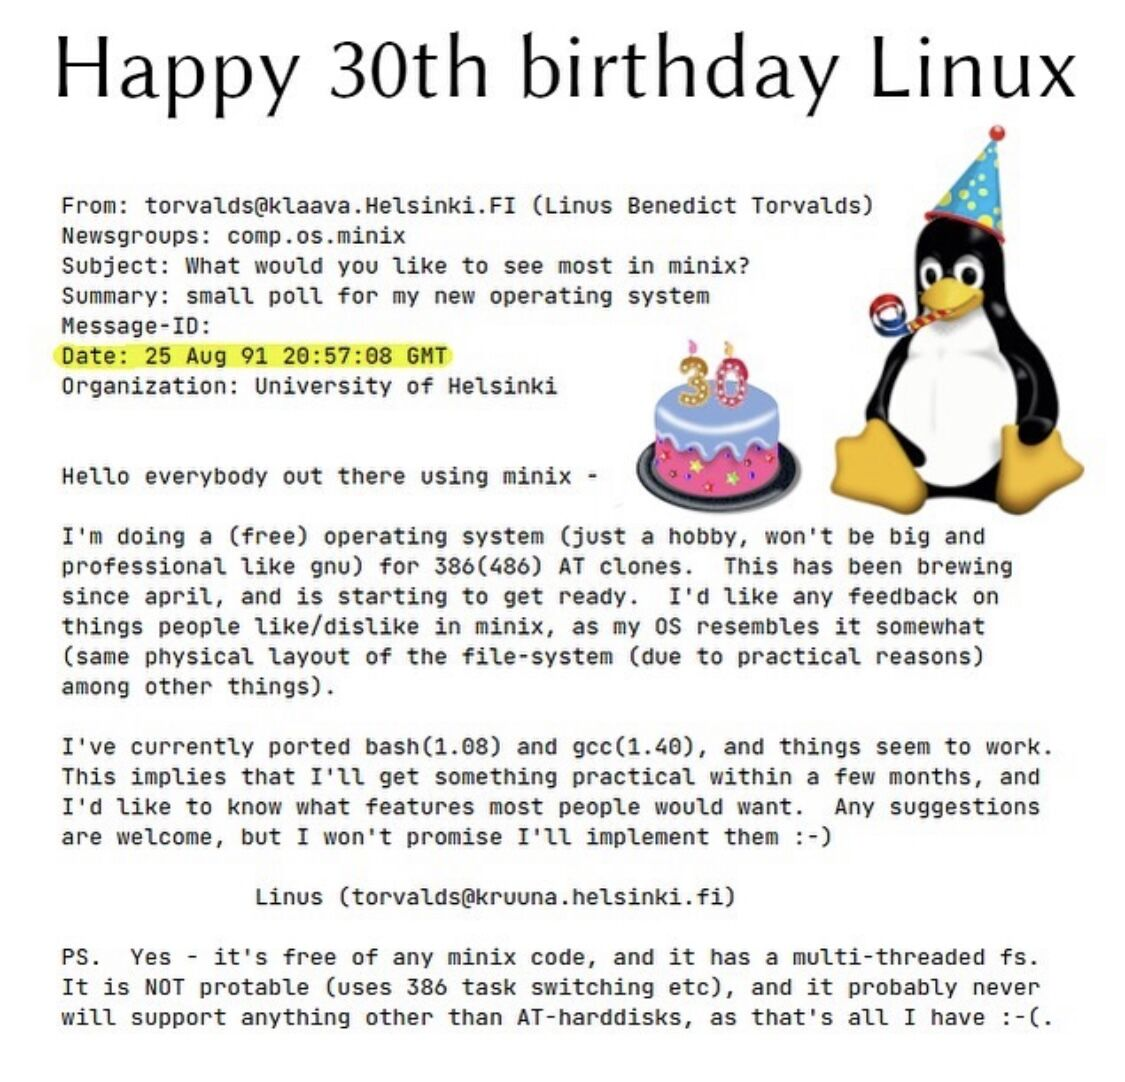
\includegraphics[scale=0.231]{Images/linux_birthday.jpg}
    }
\end{frame}

\begin{frame}{Other Unixes}
    \begin{tabular}{c c c c c}
        Unix & \$\$\$ & 1969 & Dead \\
        HP-UX & \$\$\$ & 1982 & Alive? & 
\includegraphics[scale=0.12]{L03_OperatingSystems/L3_hpux.png}\\
        SunOS & \$\$\$ & 1982 & Dead (became Solaris) \\
        AIX & \$\$\$ & 1986 & Alive \& well & 
\includegraphics[scale=0.1]{L03_OperatingSystems/L3_aix.png} \\
        Linux & Open source & 1991 & Alive \& well & 
\includegraphics[scale=0.05]{L03_OperatingSystems/L3_tux.png}\\
        Solaris & \$\$\$ $\rightarrow$ Open source & 1992 & Dead & 
\includegraphics[scale=0.14]{L03_OperatingSystems/L3_Solaris.png}\\
        FreeBSD & Open source & 1993 & Alive \& well & 
\includegraphics[scale=0.16]{L03_OperatingSystems/L3_freebsd.png}\\
        OpenBSD & Open source & 1996 & Alive \& well & 
\includegraphics[scale=0.11]{L03_OperatingSystems/L3_openbsd.png} \\
        macOS & \$\$\$ & 2001 & Alive \& well & 
\includegraphics[scale=0.11]{L03_OperatingSystems/L3_osx.jpg}
    \end{tabular}
    \vfill
    \footnotesize{Read more about Unix \& it's derivatives at \url{https://en.wikipedia.org/wiki/Unix}.} \\
    \hfill 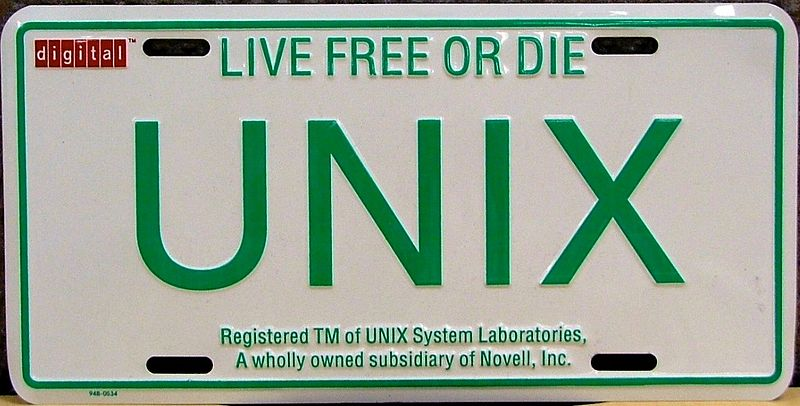
\includegraphics[scale=0.08]{L03_OperatingSystems/L3_unix_plate.jpg}
\end{frame}

\begin{frame}
    \centering
    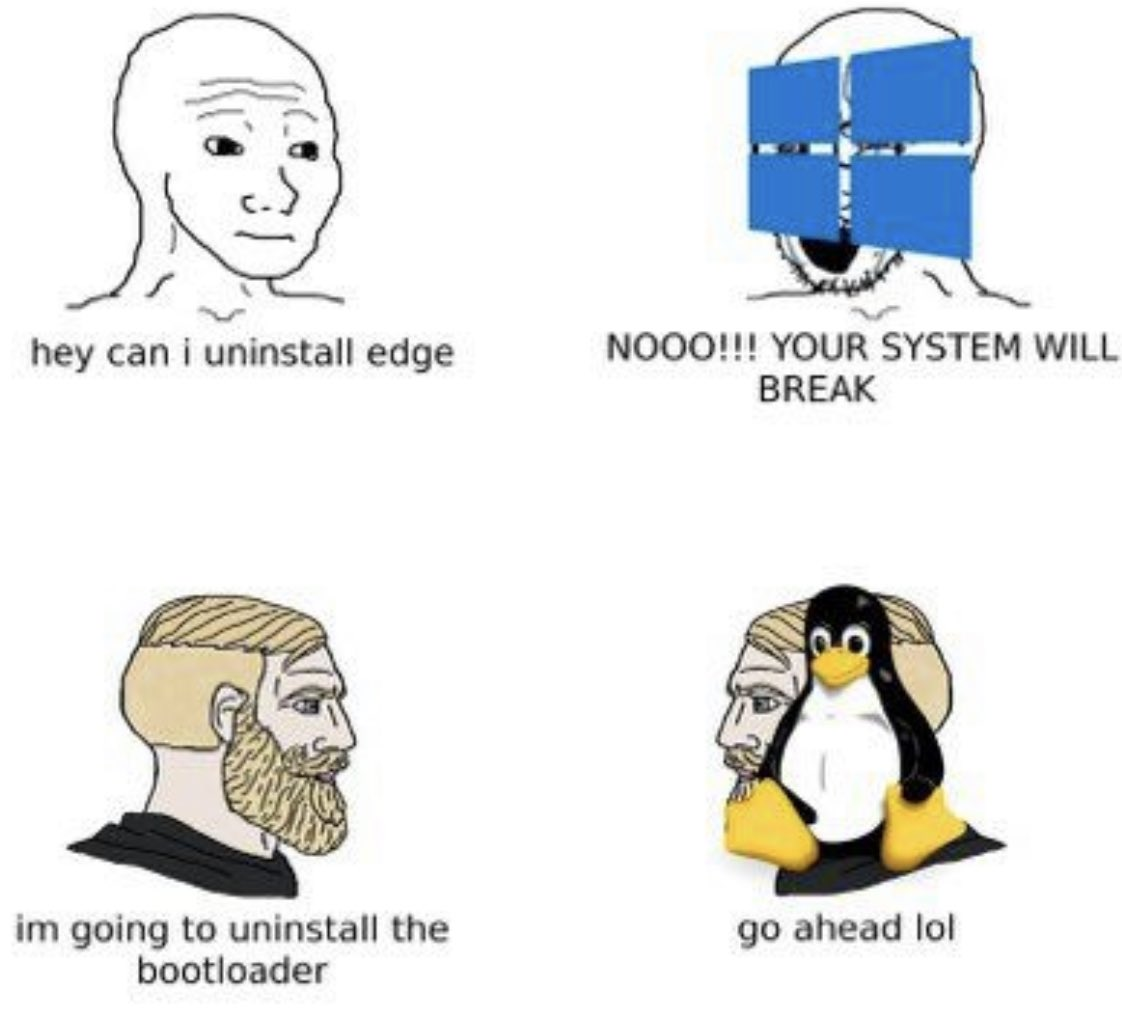
\includegraphics[scale=0.24]{Images/windows_v_linux_uninstalling.jpg}
\end{frame}

\end{document}